\section{Arrays}

Implementing arrays was definetely a challenge that required a lot of thought,
and changes in previous parts of the codebase. Some of the AST nodes needed to
store some extra information, and thus the parser had to be partially revisited.

\subsection{Parser Changes}

Although functional, array usage is quite restricted. For example, due to the
definition of the grammar, expressions arent't allowed to be used as array elements. In other words, the following
variable declaration would be syntactically incorrect:

$$ \code{let a: int[4] = [1+2, 3, 4, 5];} $$

The reason for this is that the grammar doesn't allow for expressions to be used
as array elements. This is a limitation that could be easily fixed by adding a
new rule to the grammar, but it was decided to leave it as is for the sake of
simplicity.

Furthermore, it was noted that unlike \code{Int}s, \code{Bool}s, \code{Colour}s
and \code{Float}s, the grammar doesn't offer a \code{Literal} variant for arrays.
In a function declaration, this would again be syntactically incorrect:

{\lstset{xleftmargin=0.25\textwidth}
\begin{lstlisting}
fun rot_arr() -> int[4] {
    let a: int[4] = [1, 2, 3, 4];
    return [a[1], a[2], a[3], a[0]];
}
\end{lstlisting}}

\subsection{Semantic Analysis Changes}

The semantic analysis was also updated to support arrays. The new type variant
in the \code{Type} enum $$\code{Array(Box<Type>, usize)}$$ was introduced to
represent arrays. Note that in a similar fashion to the \code{AstNode} enum, we
have to wrap the type in a \code{Box} to avoid infinite size of the \code{Type}
enum. Theoretically, this would allow the support for multi-dimensional arrays
in our type system, but that would require massive changes starting again from
the parser.

This changes allows us to hook up the type checker seamlessly, to ensure that
when arrays are passed to functions as parameters, these are checked to be of
the same type and size as the expected parameter.

\subsection{Code Generation Changes}

The code generation was also updated to support arrays. The main changes
consisted of adding the new instructions, namely \code{StoreArray},
\code{PushArray(MemoryLocation)}, \code{PushOffsetFromOpS(MemoryLocation)},
\code{PrintArray} and \code{ReturnArray}. The latter however, although available
as instruction in the VM, was not used. Even though clearly, we have seen that
functions can return arrays (although they have to be declared temporarily
inside and mutated only through direct array accesses), a slight workaround has
been implemented to achieve \textbf{properly ordered} that happens to fix other
issues that arise when referencing arrays. It was noted that some VM
instructions are inconsistent with the ordering in the storage and loading of
arrays from the operand stack.

Thus, when traversing the AST and finding an identifier which points to an
array, the following workaround occurs.
\graphicspath{figures}

\begin{figure}[H]
    \centering
    \begin{subfigure}{.5\textwidth}
        \centering
        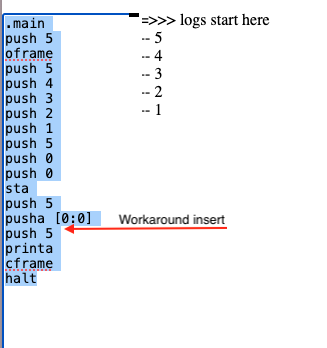
\includegraphics[width=0.6\textwidth]{figures/no_wk.png}
        \caption{Array printing without the workaround}
        \label{fig:no_wk}
    \end{subfigure}%
    \begin{subfigure}{.5\textwidth}
        \centering
        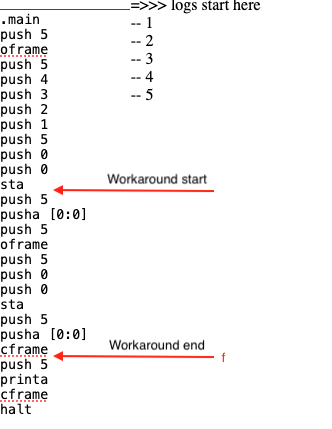
\includegraphics[width=0.5\textwidth]{figures/image.png}
        \caption{Array printing with the workaround}
        \label{fig:array_print}
    \end{subfigure}
    \caption{Inconsistent pusha and printa behaviour}
    \label{fig:array_instructions}
\end{figure}


In essence, when we find an identifier that points to an array, and call
\code{PushArray}, the contents of the array are actually pushed in reverse
order. Calling \code{PrintArray} reveals this. The workaround consists of
creating a new temporary frame with as much space as the array size, and then
store the array in the frame. Subsequently the array is pushed back to the
operand stack, but this time in the correct order. The frame is then closed and
code generation continues as usual.

Like this, wherever we use arrays, we have the guarantee that the array is
pushed in the correct order, and that it can be used anywhere as expected, even
when accessing it.
